\documentclass{article}
\usepackage[top=20mm,left=20mm,right=15mm]{geometry}
\usepackage{float}
\usepackage{graphicx}
\begin{document}


\section{Project Description}

\subsection{Detailed Methodology}

\subsubsection{Research and Problem Identification}

The project began with background research to understand how streetlights are managed in Sri Lanka . We reviewed technical articles and product datasheets to understand what components were available and suitable for our application. We also consulted with people who manage streetlights to understand the practical challenges they face. This research gave us a clear picture of the problem and helped us define the requirements for our system.



\subsubsection{Design Phase}

Based on the research and validation findings, we began the circuit design. We first identified the key functions the system needed to perform: ambient light sensing, automatic switching, current monitoring, fault detection, and alert notification. We then selected appropriate components for each function and designed the circuit in a schematic editor.

\subsubsection{Prototype Testing}

After completing the schematic, we built a prototype to test each part of the circuit separately. This allowed us to check that each component was working correctly before combining everything into a single board.

\subsubsection{PCB Design and Fabrication}

Once the prototype was tested and any issues were resolved, we created a custom PCB layout based on the schematic. The PCB was designed to be compact and organised, with clear separation between high-voltage and low-voltage sections.

\subsubsection{System Testing and Documentation}

The complete system on the PCB was tested to verify that all functions worked together correctly. We then documented our process and results in this report.

\subsection{Design and Development}

\subsubsection{System Architecture}




\begin{figure}[H]
    \centering
    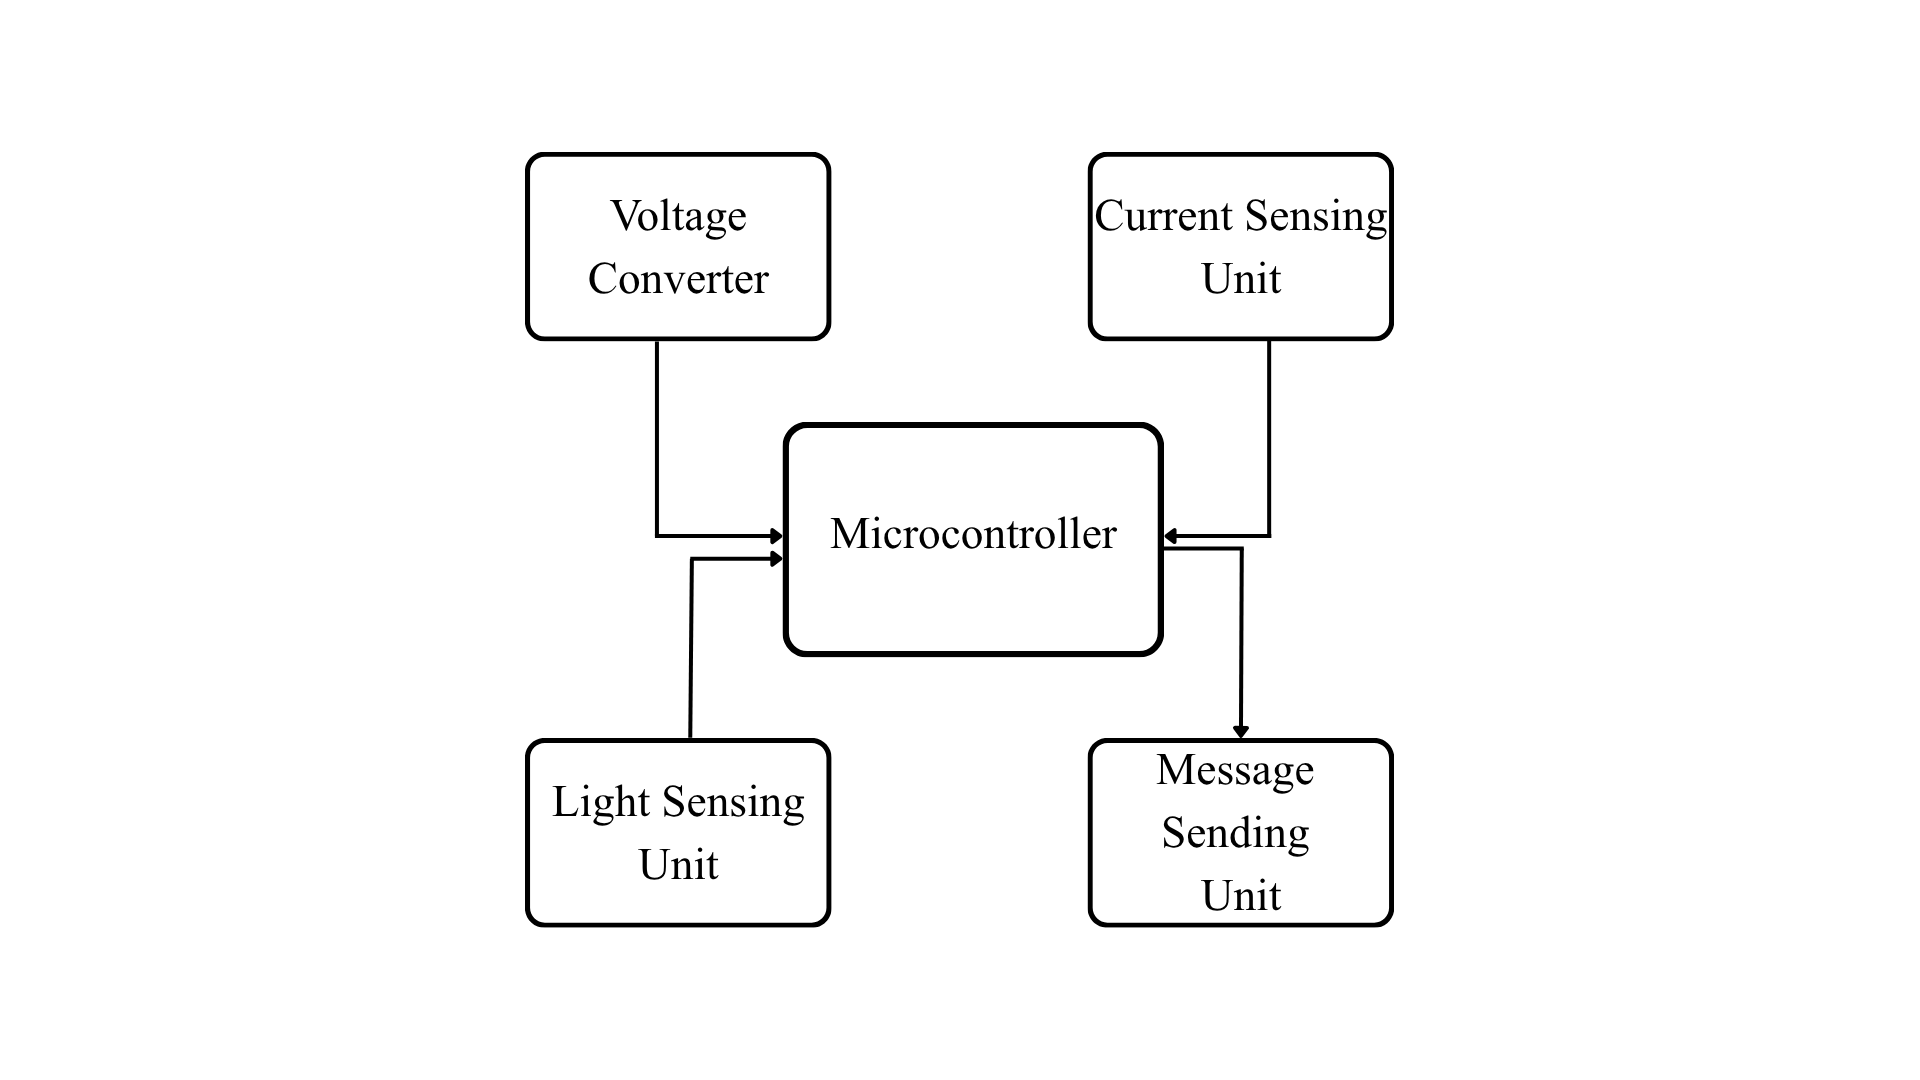
\includegraphics[width=1\textwidth]{SystemArchi.png}
    \caption{System block diagram}\label{fig:block_diagram}
\end{figure}

\subsubsection{Components}

\paragraph{ESP32-WROOM-32E}
\mbox{} \\ 

\noindent
\begin{minipage}[c]{0.4\textwidth}
    \centering
    % Replace 'esp32_image.png' with your actual image file name
    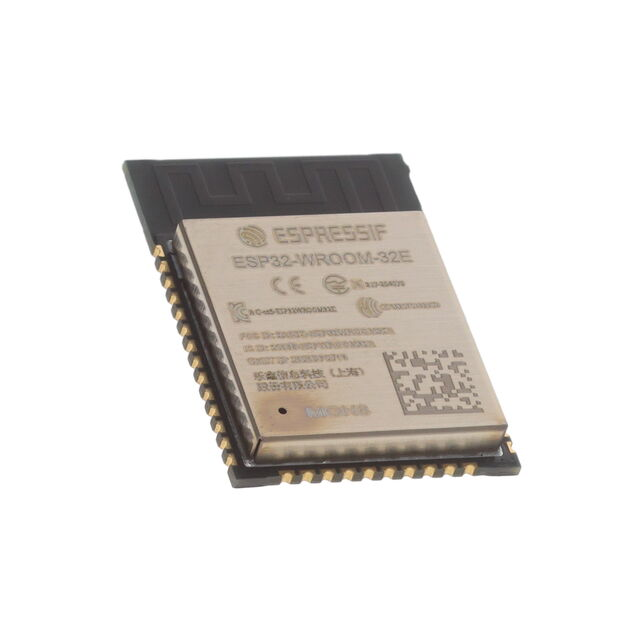
\includegraphics[width=\linewidth]{esp32.jpg} 
\end{minipage}
\hfill
\begin{minipage}[c]{0.55\textwidth}
    \begin{itemize}
        \item Serves as the main processing unit for the entire system.
        \item Built-in Wi-Fi and Bluetooth capabilities, providing room for future expansion.
        \item Analog input pins to read data from the LDR (light sensor) and the ACS712 current sensor.
        \item Digital output pin to control the relay switching.
        \item Communicates with the EVB GSM 800L module using its hardware UART serial interface.
    \end{itemize}
\end{minipage}
\paragraph{HLK-20M05}
\mbox{} \\ 

\noindent
\begin{minipage}[c]{0.4\textwidth}
    \centering
    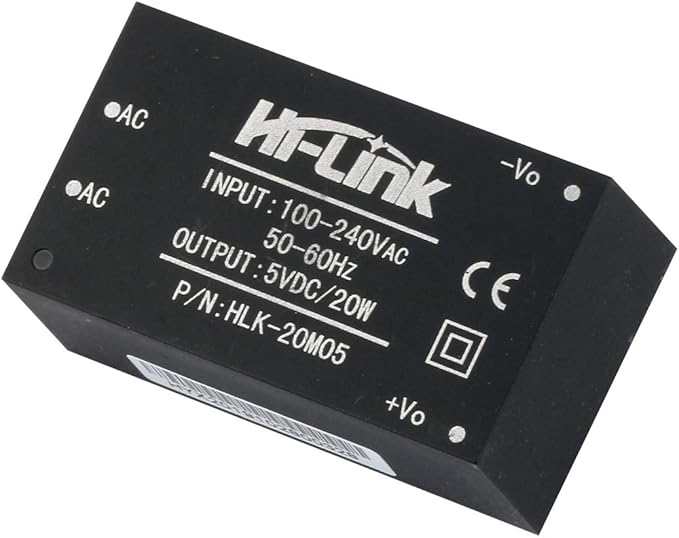
\includegraphics[width=0.5\linewidth]{HLK.jpg} 
\end{minipage}
\hfill
\begin{minipage}[c]{0.55\textwidth}
    \begin{itemize}
        \item Enclosed power module used to convert 230V AV main voltage to regulated 5V DC output with a rated current upto 4A
        \item It was choosen to power up all the components with out an external power supply 
    \end{itemize}
\end{minipage}

\paragraph{AMS1117-3.3}
\mbox{} \\ 

\noindent
\begin{minipage}[c]{0.4\textwidth}
    \centering
    % Replace 'esp32_image.png' with your actual image file name
    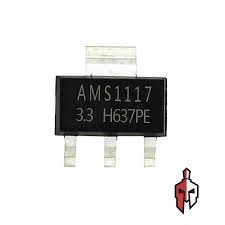
\includegraphics[width=0.75\linewidth]{AMS.jpg} 
\end{minipage}
\hfill
\begin{minipage}[c]{0.55\textwidth}
    \begin{itemize}
        \item This chip convertes 5V DC to 3.3V DC
        \item  It is a simple three-terminal device with input,output, and ground/adjust pins.
        \item  bypass capacitor (C10, 10 µF) is placed on the output to improve stability.
    \end{itemize}
\end{minipage}

\paragraph{ACS712}
\mbox{} \\ 

\noindent
\begin{minipage}[c]{0.4\textwidth}
    \centering
    % Replace 'esp32_image.png' with your actual image file name
    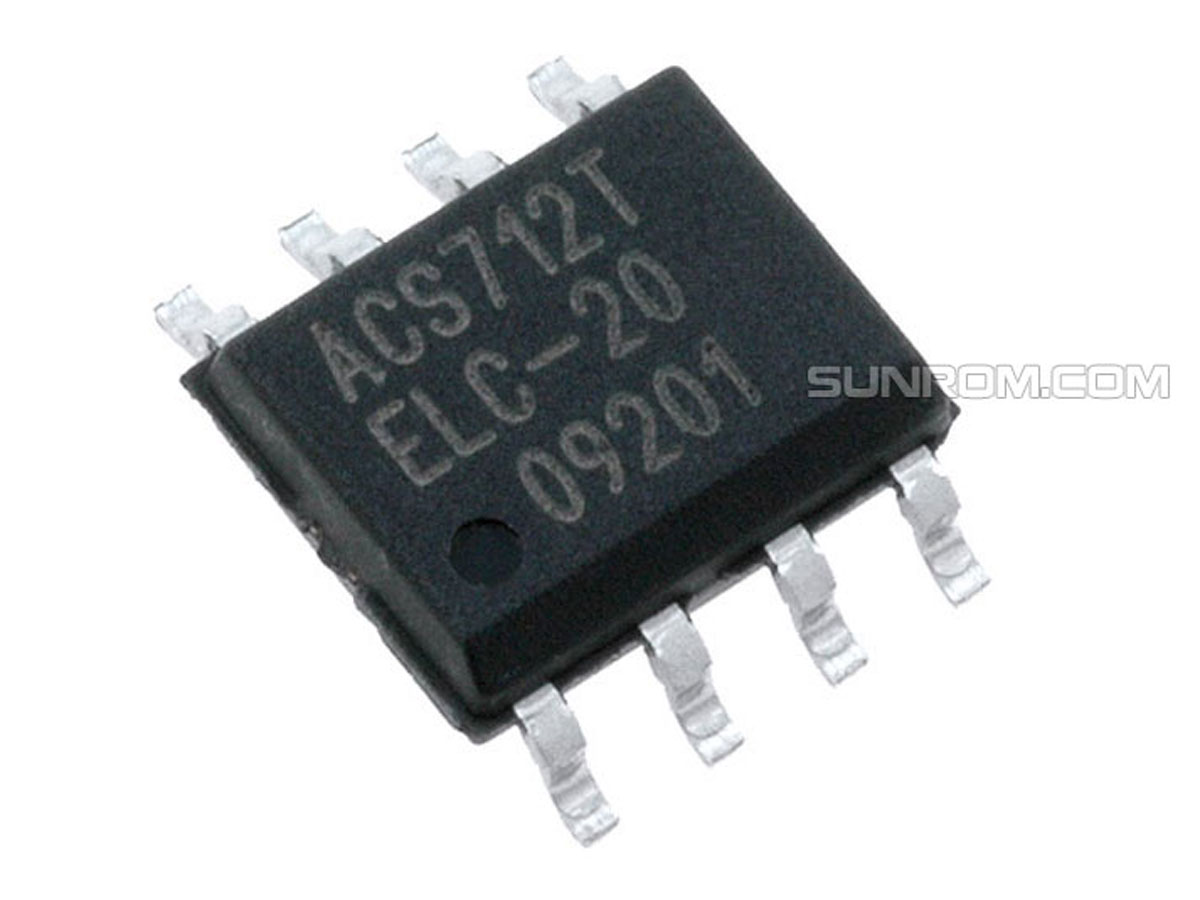
\includegraphics[width=0.5\linewidth]{ACS.jpg} 
\end{minipage}
\hfill
\begin{minipage}[c]{0.55\textwidth}
    \begin{itemize}
        \item It is a hall based current sensor module
        \item It measures the AC current flowing through thestreetlight by producing an output voltage that is proportional to the current
        \item A bypass capacitor (10\,nF) is also included to filter noise.
    \end{itemize}
\end{minipage}


\paragraph{LDR (Light Dependent Resistor)}
\mbox{} \\ 

\noindent
\begin{minipage}[c]{0.4\textwidth}
    \centering
    % Replace 'esp32_image.png' with your actual image file name
    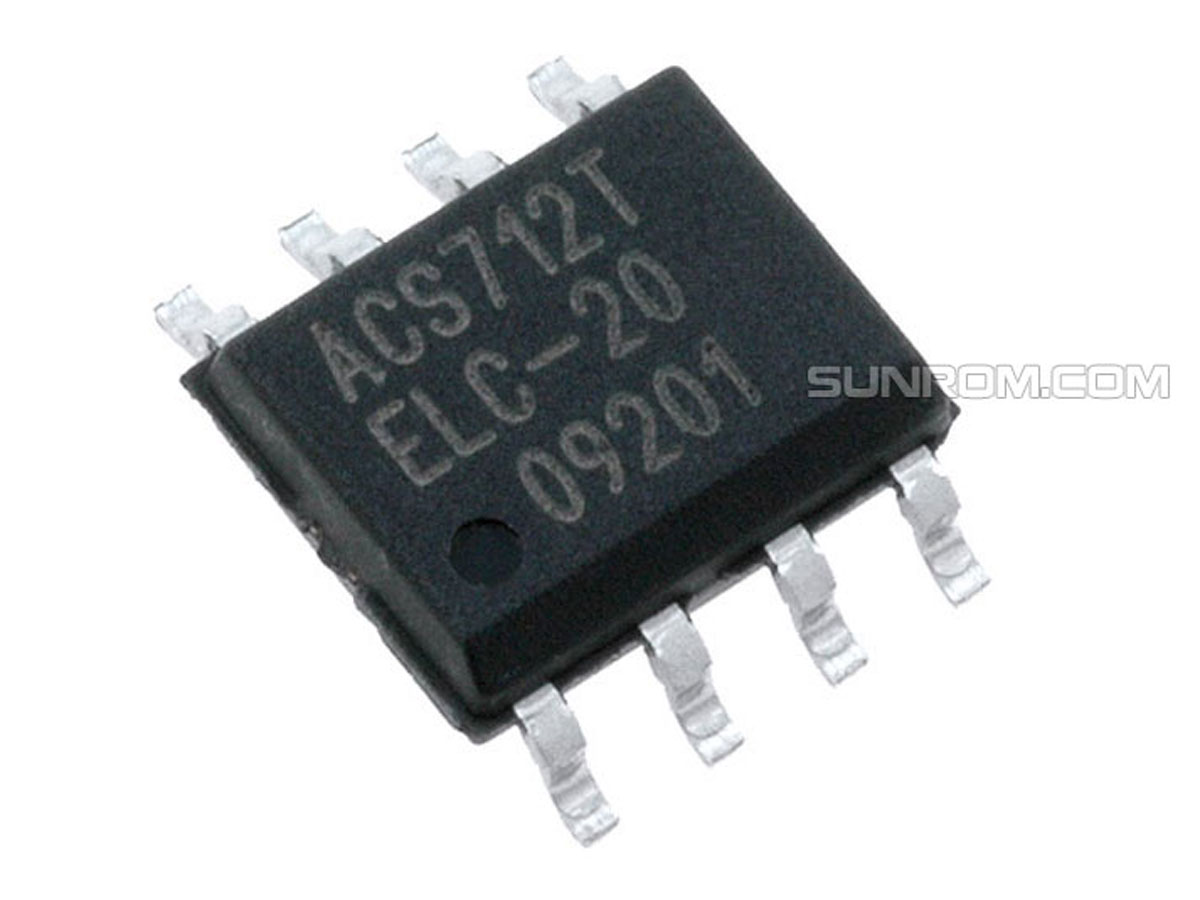
\includegraphics[width=0.5\linewidth]{ACS.jpg} 
\end{minipage}
\hfill
\begin{minipage}[c]{0.55\textwidth}
    \begin{itemize}
        \item It is used to sense light ambient level
        \item When it is dark, the resistance of the LDR increases, causing the voltage at the midpoint to change. The
microcontroller reads this voltage and determines whether the streetlight should be on or off
    \end{itemize}
\end{minipage}

\paragraph{Relay Module (K1 SRD-05VDC-SL-C)}
\mbox{} \\ 

\noindent
\begin{minipage}[c]{0.4\textwidth}
    \centering
    % Replace 'esp32_image.png' with your actual image file name
    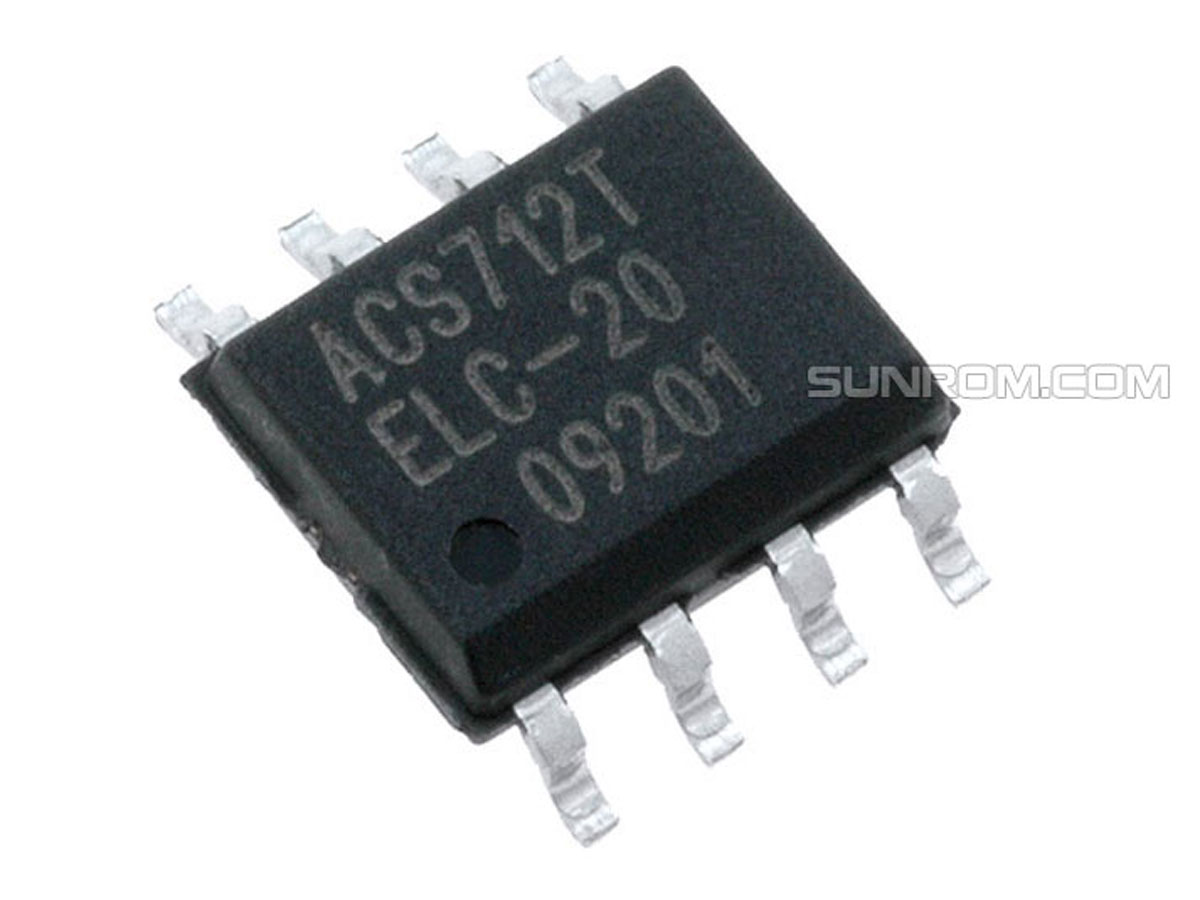
\includegraphics[width=0.5\linewidth]{ACS.jpg} 
\end{minipage}
\hfill
\begin{minipage}[c]{0.55\textwidth}
    \begin{itemize}
        \item The relay is used to switch the mains supply to the streetlight.
        \item  It is a 5V single-pole double-throw (SPDT) relay.
    \end{itemize}
\end{minipage}

 The coil of the relay is driven by a 2N2222 NPN transistor (Q1), which in turn is controlled by a GPIO pin of the ESP32 (IO\_26). A 1k$\Omega$ base resistor (R3) limits the current from the ESP32 pin into the transistor base. A 1N4007 flyback diode (D1) is connected in parallel with the relay coil to protect the transistor from the voltage spike that occurs when the relay is de-energised.

\paragraph{EVB GSM 800L Module}

The GSM module (connected via J2) is used to send SMS alerts to the maintenance team when a fault is detected. It communicates with the ESP32 over a UART serial interface using pins IO\_16 (RX of ESP32) and IO\_17 (TX of ESP32). The module operates on a 5V supply from the HLK-20M05, with 100\,$\mu$F (C6) and 1000\,$\mu$F (C7) bulk capacitors to handle the high current demand during transmission. IO\_5 is used as an additional control signal to the GSM module.

\paragraph{Supporting Passive Components}

Several passive components are used throughout the circuit to ensure stable and reliable operation:

\begin{itemize}
    \item \textbf{Decoupling capacitors} (C5, C9: 100\,nF) are placed near the power supply pins of the ESP32 to filter out high-frequency noise.
    \item \textbf{Pull-up and pull-down resistors} (R4, R5: 10k$\Omega$) are connected to the EN and IO\_0 pins of the ESP32. These ensure the microcontroller starts up in the correct state and that the boot mode is set properly.
    \item \textbf{Boot and reset buttons} (S2, S3) allow manual control of the ESP32 boot and reset functions, which are needed during programming.
\end{itemize}

\subsubsection{Circuit Design}

The circuit was designed using a schematic editor. The schematic is divided into clearly labelled functional blocks:

\begin{itemize}
    \item \textbf{230V to 5V Converter:} Contains the HLK-20M05 module and the input/output connectors.
    \item \textbf{5V to 3.3V Converter:} Contains the AMS1117-3.3 regulator and its supporting capacitors.
    \item \textbf{Relay Module:} Contains the relay K1, transistor Q1, diode D1, and resistor R3.
    \item \textbf{ACS712:} Contains the current sensor and its supporting resistors and capacitor.
    \item \textbf{LDR:} Contains the LDR and voltage divider resistor.
    \item \textbf{EVB GSM 800L:} Contains the GSM module connector and bulk capacitors.
    \item \textbf{ESP32-WROOM-32E:} The main microcontroller with all its connections.
    \item \textbf{Programming Header:} A four-pin connector for serial programming.
\end{itemize}

The complete schematic is shown in Figure~\ref{fig:schematic}.

\begin{figure}[H]
    \centering
    \fbox{\parbox{\textwidth}{\centering\vspace{2cm}\textit{Insert schematic image here}\vspace{2cm}}}
    \caption{Complete circuit schematic (Sheet1)}
    \label{fig:schematic}
\end{figure}

\subsubsection{PCB Design}

The PCB was designed based on the schematic. Several important considerations were taken into account during the layout process.

\paragraph{Layer Strategy}

A two-layer PCB was used. The top layer (shown in red in Figure~\ref{fig:pcb}) carries most of the signal and power traces. The bottom layer (shown in blue) is used for return paths and some crossing routes. Vias are used where a trace needs to change layers.

\paragraph{Trace Width}

For low-current signal traces, a standard trace width was used to minimise board area. For power supply traces carrying higher currents (especially the 5V supply line and the relay output), wider traces were used to reduce resistive voltage drops and prevent overheating.

\paragraph{Component Placement}

Components were grouped according to their function and placed close to each other to keep trace lengths short. The high-voltage section (HLK-20M05, relay, and the mains connectors) was kept physically separated from the low-voltage section (ESP32, sensors, and GSM module) to reduce the risk of interference and to meet basic safety requirements.

\paragraph{Safety Clearance}

An adequate clearance was maintained between mains-voltage traces and low-voltage traces to prevent accidental short circuits and to comply with basic electrical safety standards.

The completed PCB layout is shown in Figure~\ref{fig:pcb}.

\begin{figure}[H]
    \centering
    \fbox{\parbox{0.9\textwidth}{\centering\vspace{2cm}\textit{Insert PCB layout image here}\vspace{2cm}}}
    \caption{PCB layout (two-layer, top layer in red, bottom layer in blue)}
    \label{fig:pcb}
\end{figure}

\subsection{Implementation}

\subsubsection{Abstract Model Design}

The first step was to draw a simple block diagram of the system, showing the main functional blocks and how they connect to each other. This helped the team agree on the overall architecture before starting the detailed design.

\subsubsection{Component Selection and Circuit Construction}

After agreeing on the block diagram, the team researched and selected appropriate components for each block. The selection was based on availability, cost, operating voltage, and ease of use. Once the components were selected, the schematic was drawn. Each component was added to the schematic one block at a time, starting with the power supply, then the microcontroller, and then the peripheral components.

\subsubsection{Individual Component Testing}

Before combining everything on a single board, each component was tested individually using a breadboard prototype. This included:
\begin{itemize}
    \item Testing the LDR voltage divider to verify that the output voltage changed correctly with varying light levels.
    \item Testing the ACS712 by passing a known current and reading the output voltage.
    \item Testing the relay and transistor driver by driving the relay coil from a microcontroller GPIO pin.
    \item Testing the GSM module by sending AT commands over serial and verifying that an SMS was received.
    \item Testing the ESP32 with basic firmware to confirm that all GPIO pins were working correctly.
\end{itemize}

\subsubsection{System Integration and Full Testing}

After individual component testing, all parts were connected together and the complete firmware was uploaded to the ESP32. The system was tested as a whole to verify that:
\begin{itemize}
    \item The relay switched on when the LDR reading indicated darkness and switched off when light was detected.
    \item The ACS712 correctly detected both normal operating current and fault conditions (simulated by disconnecting the load).
    \item An SMS was sent when a fault was detected.
    \item The system recovered correctly after a fault was cleared.
\end{itemize}

\subsubsection{Transition to PCB}

Once the prototype was confirmed to be working correctly, the PCB was designed and fabricated. After receiving the PCB, components were soldered onto it and the full system was re-tested on the PCB to confirm that the PCB layout had no errors.

\subsubsection{Microcontroller Programming}

The ESP32 was programmed using the Arduino IDE with the ESP32 board support package. The firmware was structured as follows:

\begin{enumerate}
    \item \textbf{Initialisation:} Configure all GPIO pins, start serial communication with the GSM module, and set initial output states.
    \item \textbf{Main loop:} Continuously read the LDR sensor and the ACS712 sensor.
    \item \textbf{Light control:} If the LDR reading indicates darkness, turn the relay on (streetlight on). If the LDR reading indicates daylight, turn the relay off.
    \item \textbf{Fault detection:} If the relay is on but the ACS712 reading shows no current (or current below a threshold), a fault is assumed. An SMS is sent to the configured phone number with a fault alert message.
    \item \textbf{Alert management:} To avoid sending repeated SMS messages for the same fault, the system tracks whether a fault alert has already been sent and only sends a new alert when the fault condition changes.
\end{enumerate}

\subsection{Challenges and Solutions}

\subsubsection{Technical Challenges}

\paragraph{GSM Module Power Supply}

The EVB GSM 800L module requires a stable supply capable of delivering high peak currents during SMS transmission. In early testing, the module was resetting during transmission due to insufficient current supply. This was resolved by adding large bulk capacitors (100\,$\mu$F and 1000\,$\mu$F) close to the module's power supply pins, which store charge and supply the peak current needed during bursts of transmission activity.

\paragraph{ACS712 Noise}

The output of the ACS712 contains some noise, which caused occasional false fault readings. This was addressed by averaging several ADC readings in the firmware before making a fault decision, which effectively filtered out the noise.

\paragraph{LDR Threshold Sensitivity}

The threshold light level at which the relay should switch was difficult to set correctly, because the ambient light level varies with weather and location. We resolved this by making the threshold value a configurable parameter in the firmware, which can be adjusted without changing the hardware.

\paragraph{Mains Voltage Safety}

Working with 230V mains voltage required careful attention to safety during testing. We took precautions by testing the high-voltage section only after confirming that the low-voltage section was working correctly, and by using appropriate insulation and safety practices throughout.

\subsubsection{Non-Technical Challenges}

\paragraph{Component Availability}

Some components were not available locally and had to be ordered online, which caused delays. We addressed this by ordering components early and keeping spare parts for critical components.

\paragraph{Budget Management}

The cost of components exceeded our initial estimate, primarily due to the cost of the GSM module and the PCB fabrication. We managed this by reducing the number of prototype iterations and carefully planning the PCB layout to avoid the need for redesigns.

\paragraph{Team Coordination}

Coordinating the work among team members was at times challenging, particularly when some members were working on different aspects of the project simultaneously. We addressed this by holding regular meetings and using a shared document to track progress.
\end{document}